\documentclass[border=16pt]{standalone}
\usepackage{tikz}
\usetikzlibrary{arrows.meta, positioning}
\begin{document}
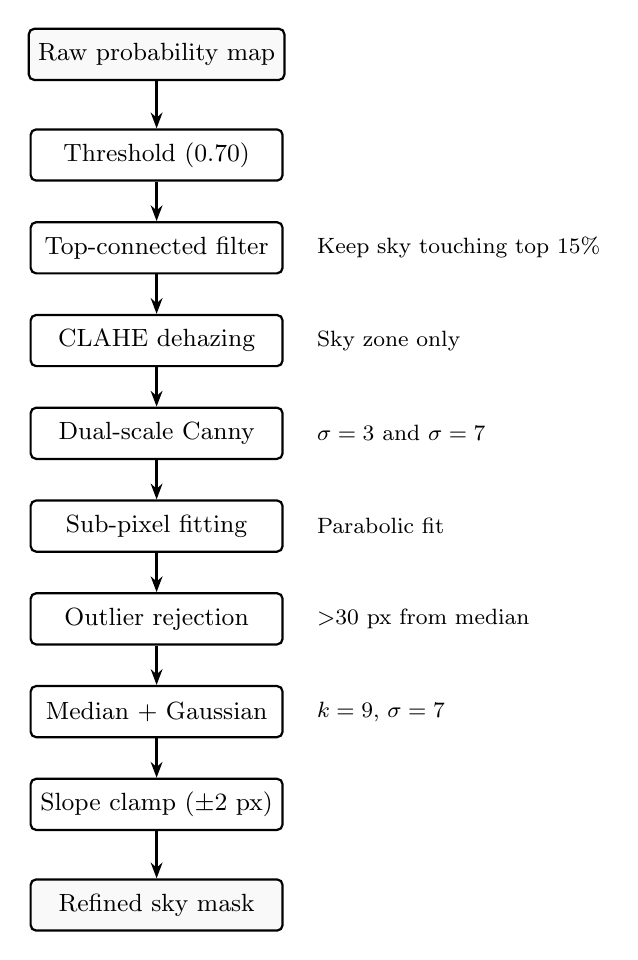
\begin{tikzpicture}[
    node distance=0.55cm and 0.8cm,
    box/.style={rectangle, draw=black, thick, minimum width=3.2cm, minimum height=0.65cm,
                text centered, font=\small, rounded corners=2pt},
    io/.style={rectangle, draw=black, thick, minimum width=3.2cm, minimum height=0.65cm,
               text centered, font=\small, rounded corners=2pt, fill=gray!5},
    arr/.style={-{Stealth[length=2mm]}, thick},
]

% Input
\node[io] (in) {Raw probability map};

% Steps
\node[box, below=0.6cm of in] (th) {Threshold (0.70)};
\node[box, below=0.5cm of th] (tc) {Top-connected filter};
\node[box, below=0.5cm of tc] (cl) {CLAHE dehazing};
\node[box, below=0.5cm of cl] (ca) {Dual-scale Canny};
\node[box, below=0.5cm of ca] (sp) {Sub-pixel fitting};
\node[box, below=0.5cm of sp] (or) {Outlier rejection};
\node[box, below=0.5cm of or] (sm) {Median + Gaussian};
\node[box, below=0.5cm of sm] (sc) {Slope clamp ($\pm$2 px)};

% Output
\node[io, below=0.6cm of sc] (out) {Refined sky mask};

% Arrows
\draw[arr] (in) -- (th);
\draw[arr] (th) -- (tc);
\draw[arr] (tc) -- (cl);
\draw[arr] (cl) -- (ca);
\draw[arr] (ca) -- (sp);
\draw[arr] (sp) -- (or);
\draw[arr] (or) -- (sm);
\draw[arr] (sm) -- (sc);
\draw[arr] (sc) -- (out);

% Side notes
\node[font=\footnotesize, right=0.3cm of tc] {Keep sky touching top 15\%};
\node[font=\footnotesize, right=0.3cm of cl] {Sky zone only};
\node[font=\footnotesize, right=0.3cm of ca] {$\sigma=3$ and $\sigma=7$};
\node[font=\footnotesize, right=0.3cm of sp] {Parabolic fit};
\node[font=\footnotesize, right=0.3cm of or] {$>$30 px from median};
\node[font=\footnotesize, right=0.3cm of sm] {$k=9$, $\sigma=7$};

\end{tikzpicture}
\end{document}
